\documentclass[12pt]{article}
\usepackage{graphicx}
%%%%%%%%%%%%%%%%%%%%%%%%%%%%%%%%%%%%%%%%%%%%%%%%%%%%%%%%%%
\begin{document}
\begin{center}
{\huge Python  Final  Project  Write-Up}
  \vspace{5 mm}

by: Brian Valtin
\end{center}
%%%%%%%%%%%%%%%%%%%%%%%%%%%%%%%%%%%%%%%%%%%%%%%%%%%%%%%%%%
\section{Abstract}
For our final project in CSIS 200 our goal is to predict rainfall that will occur in a month, whether that being how often it will be occuring or how much of it is going to fall. The first part that we had to predict is how often it would rain in a given month and then come up with a probability that fit a certain condition. Our first problem was that we had to predict the odds that it would only rain once a month with a 20 percent chance that it would rain every day. We had to approach this problem using a Monte Carlo approach generating random numbers and we had a condition that every month had 30 days in it. After solving the problem I came up with that there is about a 0.9 percent chance that it would rain once and only once in a given month. The second problem was similar to the first, although this time there were new conditions. There were still the same days in every month, but this time there was a only a 10 percent chance that it would rain on any given day in the month. For this problem we had to calculate the odds that it would rain at least 8 days in a month. Once again, we had to work out this problem numerically using a Monte Carlo approach to it. After solving it I came up with that there is about a 0.8 percent chance that it would rain at least 8 days in a month. The third problem had us predicting the amount of rainfall that would occur in a month under certain conditions. If it was the first day of the month there is a 10 percent chance that it will rain. If it rained one day before, but not 2 days before there is a 20 percent chance that it'll rain. If it rained both the 2 days before, but not the third there is a 25 percent chance that it'll rain. If it rained all 3 days before there is a 5 percent chance that it will rain. Otherwise there is only a 10 percent chance that it'll rain. We needed to find out what the odds are that at least 10 cm of rain falls in a given month using a Monte Carlo approach. After solving the problem I got a probability of about 46 percent.
%%%%%%%%%%%%%%%%%%%%%%%%%%%%%%%%%%%%%%%%%%%%%%%%%%%%%%%%%%%
\section{Introduction}
Our final project had to do with predicting rainfall and the probability that cetain amounts of rainfall or days of rainfall will occur. The overall goal of the project was to calculate probability using a Monte Carlo approach that would give the probability that a cerain event would occur under certain conditions. Every problem there were new and different conditons that had to be accounted for in order to calculate the correct probability.
%%%%%%%%%%%%%%%%%%%%%%%%%%%%%%%%%%%%%%%%%%%%%%%%%%%%%%%%%%%  
\section{Problem 1}
\subsection{Analytic Solution}
$$ x = (30*0.2^n*0.8^{30-n})*100$$
\begin{center}
n = amount of days it rains in the month (1 day)
\end{center}
$$ x = (30*0.2^1*0.8^{29})*100$$
$$ x = 0.93\%$$
\subsection{Code Explanation}
Before I started trying to think of any code I should be using I imported numpy into the code since a Monte Carlo approach was necessary in order to solve the problem numerically. First, I initallized some variables that stood for the the amount to months that I was looping over, the amount of days in a month, and initialized a tracker that will track how many months it rained once and only once. I then began a loop that looped the amount of months that I programed my code to run. For every month my code looped over a list of random numbers I generated to represent if it would rain on a given day. I set a tracker that tracks the amount of times it rained every month. It would track every time a 3 showed up on my random number generator when I generated a set of 30 random numbers ranging from 1 to 5. There is a 20\% chance that a 3 will show up on the list representing the 20\% chance it has to rain on any given day. If the rain tracker only read one 3 during a month I would add 1 to the tracker that tracked the amount of months it only rained once. Once all the months looped over I found the probability that it would rain once a month by dividing the amount of months that it only rained once by the total amount of months and multiplied the result by 100 to get a percentage. My result of this problem was that there was about a 0.9\% chance that it would only rain once in a month if there was a 20\% chance that it would rain everyday.
%%%%%%%%%%%%%%%%%%%%%%%%%%%%%%%%%%%%%%%%%%%%%%%%%%%%%%%%%%%
\section{Problem 2}
I approached this problem similarly to the way I completed Problem 1. I once again made some variables that represented the amount of months I was looping over, as well as a new tracker that tracked every time it rained 8 or more times in a month. Like the last problem, I looped the amount of months that I programmed my code to run. In that loop I set a new tracker that tracked the amount of times it rained per month. I did this by generating a list of 30 random numbers between 1 and 10 and tracked every time a 3 came up on that list. There is as 10\% chance that a 3 appears on the list that represents the 10\% chance that it has to rain every day in the month. If the raintracker is 8 or greater then it adds to the amount of months that it rains more than 8 times. Once all the months have looped over I find the probability by dividing the number of months it rained more than 8 times by the total amount of months and multiplied the result by 100 to get a percentage. My result for this problem was that there was about a 0.8\% chance that it would rain 8 or more times in a month if there was a 10\% chance that it would rain on a particular day.
%%%%%%%%%%%%%%%%%%%%%%%%%%%%%%%%%%%%%%%%%%%%%%%%%%%%%%%%%%%%
\section{Problem 3}
\subsection{3A}
The first thing I did when approaching this problem was I created a function that would calculate the amount of rainfall that would occur if it were to rain that day. In this function I created a variable that would store the amount of rain that fell and returned it in the end. To get the amount of rain that fell I generated a random number between 1 and 10. If the random number was a 1 or a 2 the amount of rain that fell would be 1 cm. The one and the two represent the 20\% chance that it had to rain 1 cm. If the random number was a 3, 4, or 5 the amount of rain that fell would be 2 cm. The three, four, and five represent the 30\% chance that it had to rain 2 cm. If the random number was a 6, 7, or 8 the amount of rain that fell would be 3 cm. The six, seven, and eight represent the 30\% chance that it had to rain 3 cm. If the random number was a 9 the amount of rainfall would be 4 cm. The nine represents the 10\% chance that it had to rain 4 cm. If the random number was a 10 the amount of rainfall would be 5 cm. The ten represents the 10\% chance that it had to rain 5 cm.

I then created a new function that would figure out how many months it rained 10 or more cm and find out what the probability was that it were to rain that much. To start the function I initialized some variables that represented the amount of months that I was looping over, the amount of days in a month, as well as the amount of months that it rained 10 cm or more. Then I started the loop over the months that I set to run and initialized a variable to track the amount of rainfall occured that month. To represent the first senario that there was a 10\% chance that it would rain on the first day of the month I generated a random number between 1 and 10 and tracked whenever a 3 appeared which represented the 10\% chance that it would occur. If a 3 did come up I ran through my amount of rainfall function that calculated how much it rained that day and added it to the rain total. If that senario occurred I moved on the next senario which was if it rained one day before, but not the second or third then there was 20\% chance of rain. First I generated a list of random numbers between 1 and 5 and tracked whenever a 3 appeared to represent the 20\% chance it had to occur. If that 3 appeared then I ran my amount of rainfall function and added the result to the total amount of rainfall for that month. If that senario happened I moved on the next one that if it rained the last 2 days, but not the third then there was  a 25\% chance of rain. To accomplish this I generated a list of random numbers that were between 1 and 4 and tracked whenever there was a 3 to represent the 25\% chance it had to rain. If this condition was met then I ran my amount of rainfall function and added the result to my total rainfall for the month. If this senario was met then I moved on the next one which stated that if it rained the past 3 days then there was a 5\% chance that it would rain that day. To find out if it rained I generated a list of random numbers between 1 and 20 and tracked whenever there was a 3 to represent the 5\% chance that it had of raining that day. If this happened then I ran my amount of rainfall function and added that result to my total amount of rainfall for that month. If any of these senarios failed to happen during this then it would reset back to the original that there was a 10\% chance that it would rain anyday which was the last senario. It worked the same as the first senario for the first of the month. Once it looped through all the days in the month it would see if the total amount of rainfall was greater than or equal to 10 then would add one to the variable that tracked if it rained 10 cm or more in a month. Once all the months ran through I divided the amount of months it rained 10 cm or more by the total amount of months and multiplied it by 100 to find the percentage and returned that value.
\subsection{3B}
To create the histogram of the amount of rainfall that occured in a day that it rained first I imported matplotlib and made it appear in the notebook. Then I created a variable that represented the amount of days it was looping over. Then I created an empty list and ran my function the amount of times as the days I set to and appended the values into the list. Then I created the figure that had a range of 1 to 6 and had 5 bins. I labeled the x axis "Amount of Rainfall" and labeled the y axis "Number of Days". Then the code went through the list and plotted the results.

\begin{figure}[h]

\centering
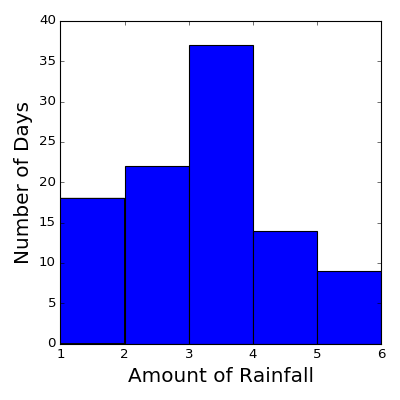
\includegraphics[width=0.5\textwidth]{Histogram.png}
\caption{Histogram of amount of rainfall per day it rains \label{Histogram}}
\end{figure}  
\end{document}







